% id: 17-20
% book: 베이직쎈 확률과 통계 · 01 여러 가지 순열
% section: 유형 010 최단 거리로 가는 경우의 수; 중간 지점을 잡아야 하는 경우
% figure: tikz:fig-17-20
% answer: 
% answer_source: 
% variant_level: 0 (원본 전사)
% 이 파일은 build.mjs 가 items.json 에서 만든다. 고칠 때는 items.json 을 고친다.
\smash{\raisebox{1.5mm}{\dmkichul{베이직쎈 확률과 통계 17쪽 20번}}}
\noindent\begin{minipage}[t]{0.58\linewidth}\vspace{0pt}\raggedright 오른쪽 그림과 같은 도로망이 있다. $\pt{A}$에서 $\pt{B}$까지 최단 거리로 가는 경우의 수를 구하시오.\end{minipage}\hfill\begin{minipage}[t]{0.4\linewidth}\vspace{0pt}\centering \resizebox{\ifdim\width>\linewidth\linewidth\else\width\fi}{!}{% 17-20(본책 17쪽) — 가로 3칸·세로 5칸 도로망에서 가운데 왼쪽 두 칸 넓이만큼 도로가 없는 그림(왼쪽에서 둘째 세로줄은 위 1칸과 아래 2칸만, 위에서 셋째 가로줄은 오른쪽 1칸만 있다). A 왼쪽 위 · B 오른쪽 아래. 스캔 그림을 TikZ 로 다시 그림(스캔 화질).
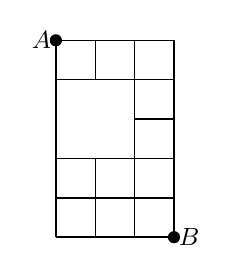
\begin{tikzpicture}[line width=0.5pt]
  % 가로줄 — 위에서 셋째(y=1.5)만 오른쪽 한 칸
  \foreach \y in {0, 0.5, 1, 2, 2.5} { \draw (0,\y) -- (1.5,\y); }
  \draw (1,1.5) -- (1.5,1.5);
  % 세로줄 — 왼쪽에서 둘째(x=0.5)는 위 1칸과 아래 2칸만
  \foreach \x in {0, 1, 1.5} { \draw (\x,0) -- (\x,2.5); }
  \draw (0.5,2) -- (0.5,2.5);
  \draw (0.5,0) -- (0.5,1);
  \fill (0,2.5) circle (2.2pt);
  \node[left, font=\small, inner sep=1.5pt] at (0,2.5) {$\pt{A}$};
  \fill (1.5,0) circle (2.2pt);
  \node[right, font=\small, inner sep=1.5pt] at (1.5,0) {$\pt{B}$};
\end{tikzpicture}
}\end{minipage}\par
